% -----------------------------------------------------------------------------
\subsection{Description of Discriminating Variables used in the \lephad
  Channels}%
\label{app:lephad_mva_variables}
% -----------------------------------------------------------------------------

A description of the discriminating variables used in the \lephad channel is
given (see also \Cref{sec:mva_discriminating variables} and
\Cref{tab:mva_inputvar}). Reconstructed electrons and muons are collectively
referred to as leptons~($\ell$), hereafter.
\begin{description}

\item[$\Delta \pT(\ell, \tauhadvis)$] The transverse momentum difference between
  lepton and \tauhadvis.

\item[\mTW] The transverse mass of the lepton and \pTmiss defined as
  \begin{align*}
    \mTW = \sqrt{2 |\myvec{p}_{\text{T}}^{\ell}| |\pTmiss| \cos(1 -
    \Delta\phi)} \,\text{,}
  \end{align*}
  where $\Delta\phi$ is the angle between \pTmiss and
  $\myvec{p}_{\text{T}}^{\ell}$.

\item[\pTmiss $\phi$ centrality] A measure of the relative angular position of
  \pTmiss and visible \taulepton decay products (electrons, muons, or
  \tauhadvis) in the transverse plane. It is defined as
  % The measurement is relative to the line bisecting the azimuthal angle
  % between the pair of visible \taulepton decay products and is defined
  % as~\cite{HIGG-2013-32, HIGG-2016-16-witherratum}:
  \begin{align*}
    \pTmiss\text{ }\phi\text{ centrality} = \frac{A + B}{\sqrt{A^2 + B^2}} \text{,}
  \end{align*}
  where
  \begin{align*}
    A = \frac{\sin(\phi_{\pTmiss} - \phi_{\tau_1})}{\sin(\phi_{\tau_2} - \phi_{\tau_1})} \qquad B = \frac{\sin(\phi_{\tau_2} - \phi_{\pTmiss})}{\sin(\phi_{\tau_2} - \phi_{\tau_1})} \text{,}
  \end{align*}
  with $\phi_{\pTmiss}$ and $\phi_{\tau_1}$/$\phi_{\tau_2}$ denoting the
  azimuthal angle of \pTmiss and visible \taulepton decay products,
  respectively~\cite{HIGG-2013-32, HIGG-2016-16-witherratum}.

  The \pTmiss $\phi$ centrality is defined relative to the line bisecting the
  azimuthal angle spanned by the visible \taulepton decay products. It reaches a
  maximum of $\sqrt{2}$ (minimum of $-\sqrt{2}$) when \pTmiss is aligned with
  the bisecting line and pointing into the smaller (larger) angle defined by the
  decay products. In configurations where \pTmiss is collinear with one of the
  visible \taulepton decay products it takes a value of 1.

\item[$\Delta\phi(\ell\tauhadvis, bb)$] Azimuthal angle between the
  $\ell + \tauhadvis$ system and the system consisting of the two \bjet
  candidates.

\item[$\Delta\phi(\ell, \pTmiss)$] Azimuthal angle between the lepton and
  \pTmiss.

\item[$\Delta\phi(\pTauTau, \pTmiss)$] Azimuthal angle between
  $\tau\tau$-system, reconstructed using the MMC, and \pTmiss.

\item[$s_{\text{T}}$] The scalar sum of transverse momenta of all selected jets,
  \tauhadvis, leptons, and \pTmissAbs.

\end{description}


% -----------------------------------------------------------------------------
\clearpage
\subsection{Correlation Matrices of the MVA Input Variables in the \hadhad
  Channel}
% -----------------------------------------------------------------------------

\begin{figure}[htbp]
  \centering

  \begin{subfigure}[t]{.49\textwidth}
    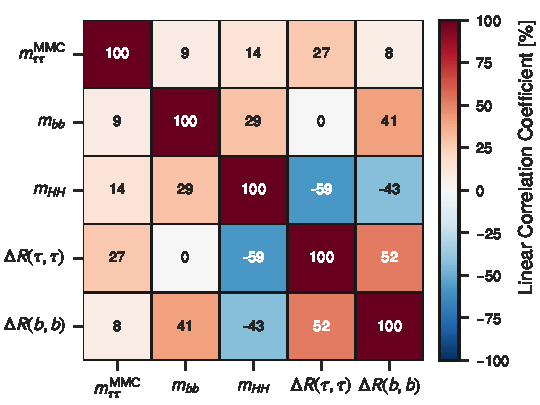
\includegraphics[width=\textwidth]{mva/correlations/NonResHH_pearson}
    \subcaption{SM~\HH production via \ggF}
  \end{subfigure}\hfill %
  \begin{subfigure}[t]{.49\textwidth}
    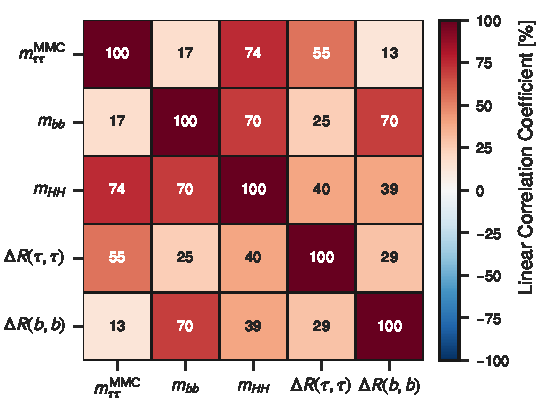
\includegraphics[width=\textwidth]{mva/correlations/ttbar_pearson}
    \subcaption{Top-quark pair production}
  \end{subfigure}

  \begin{subfigure}[t]{.49\textwidth}
    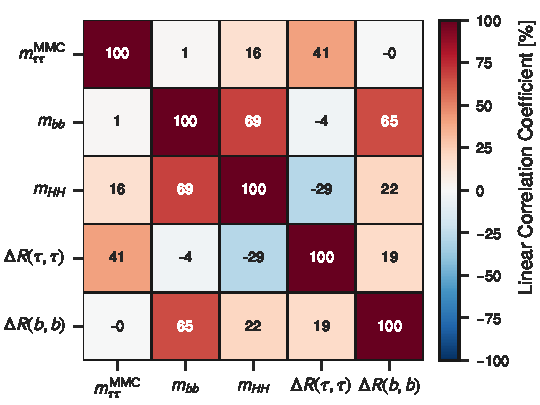
\includegraphics[width=\textwidth]{mva/correlations/Ztautau_pearson}
    \subcaption{$Z \rightarrow \tautau + \text{jets}$}
  \end{subfigure}\hfill %
  \begin{subfigure}[t]{.49\textwidth}
    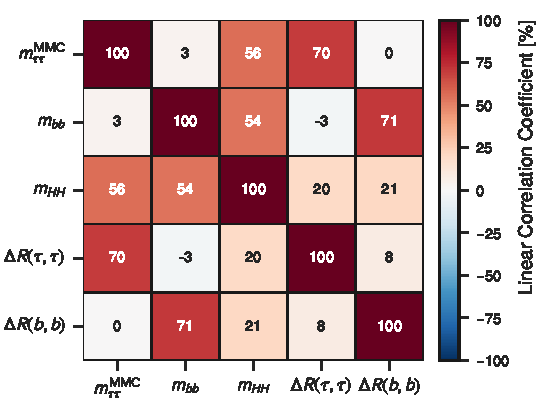
\includegraphics[width=\textwidth]{mva/correlations/Fake_pearson}
    \subcaption{Multi-jet}
  \end{subfigure}

  \caption[Correlation coefficients between the MVA input variables used in the
  \hadhad channel.]{Correlation coefficients between the MVA input variables
    used in the \hadhad channel. The correlation matrices are shown separately
    for the SM~\HH signal (a) and the three largest backgrounds in the \hadhad
    SR (b-d).}%
  \label{fig:mva_input_correlations}
\end{figure}


% ------------------------------------------------------------------------------
\clearpage
\subsection{Discrimination Power of the PNN as a Function of \mX in the \hadhad
  Channel}%
\label{app:pnn_rocauc_vs_mx}
% ------------------------------------------------------------------------------

\begin{figure}[htbp]
  \centering

  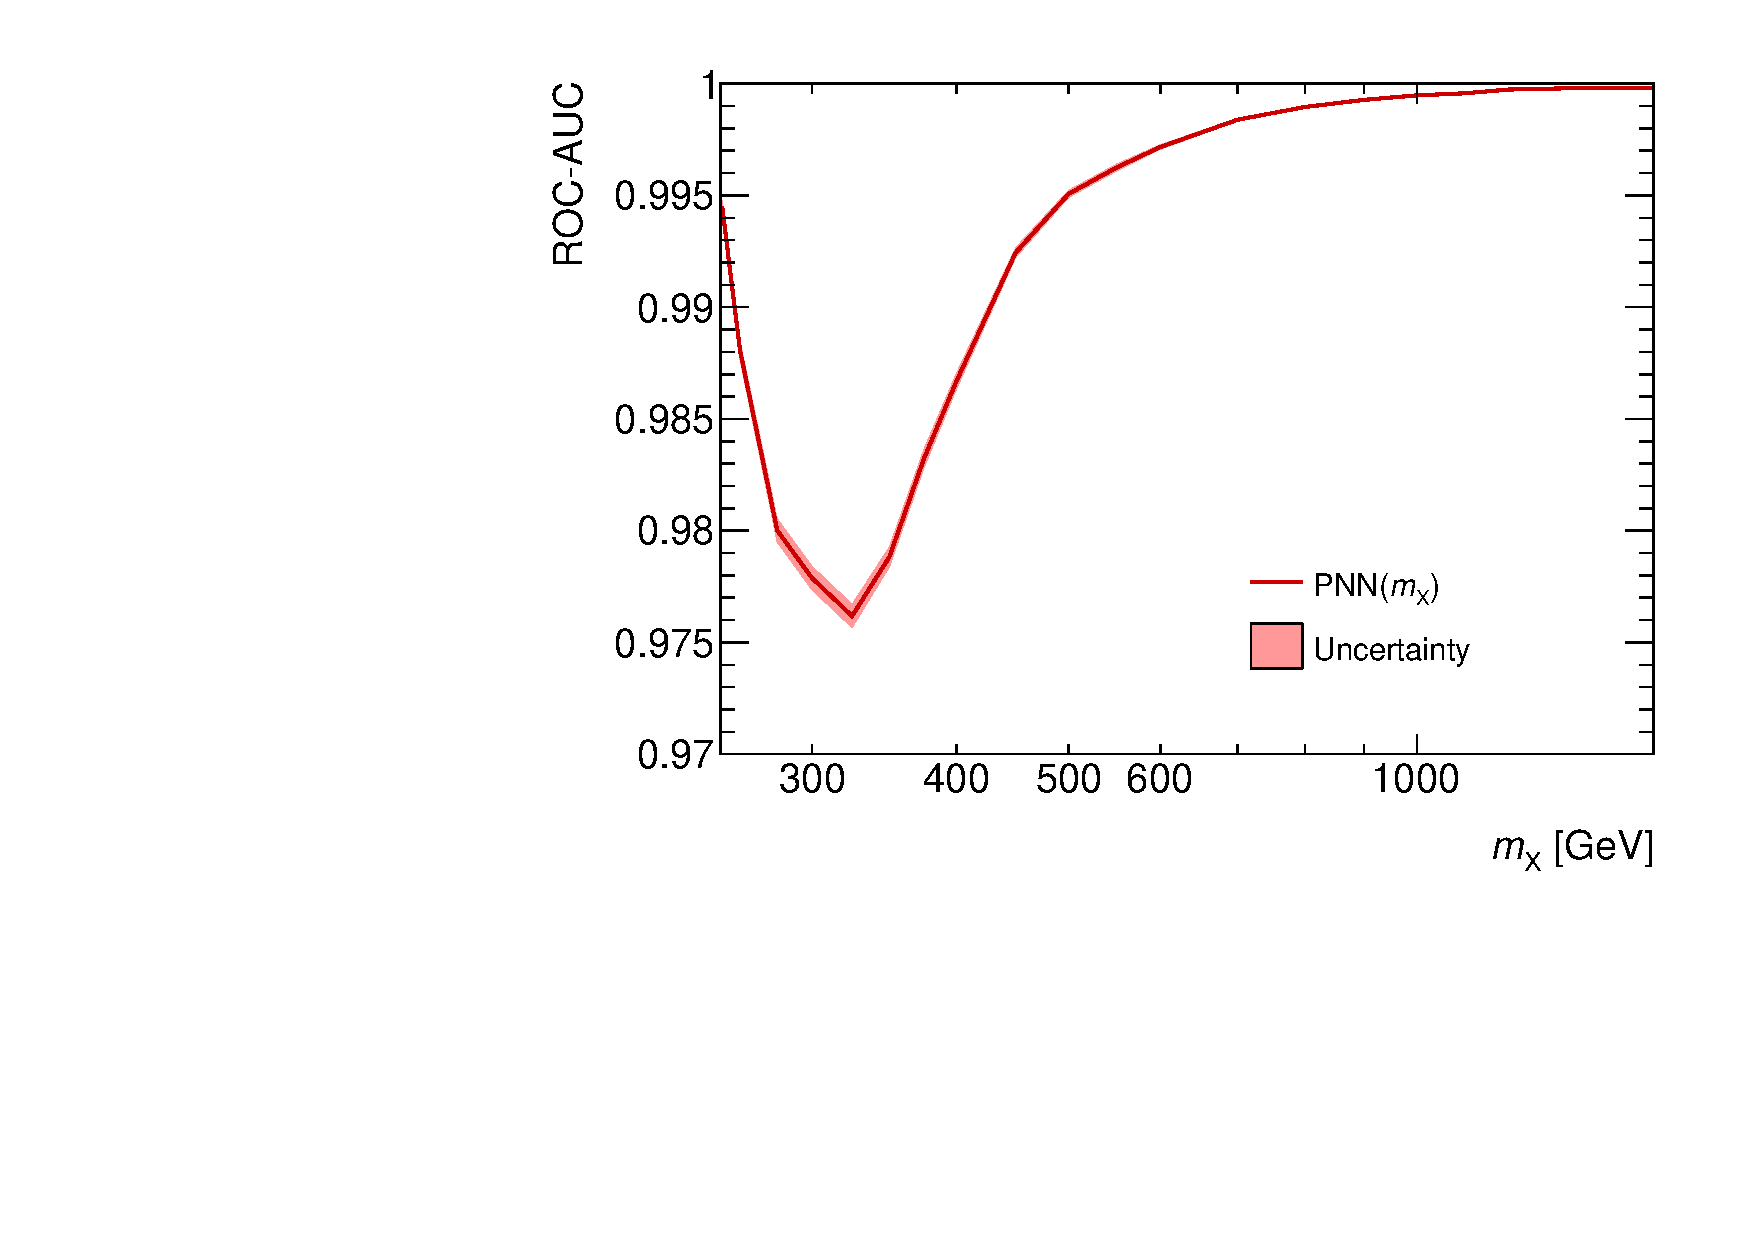
\includegraphics[width=0.65\textwidth]{mva/rocauc_vs_mx}

  \caption[ROC-AUC.]{Area under the receiver operating characteristic curve
    (ROC-AUC) for the PNN discriminant in the \hadhad channel. The ROC-AUC is
    calculated for the binary classification task of distinguishing signal
    events (i.e.\ resonant \HH production via resonances of mass \mX) from
    background events in the \hadhad SR. Only statistical uncertainties from the
    finite number of simulated and CR events is shown.}%
  \label{fig:pnn_rocauc_vs_mx}
\end{figure}


%%% Local Variables:
%%% mode: latex
%%% TeX-master: "../../phd_thesis"
%%% End:
